\chapter{Blinn-Phong Lighting}

In this chapter we add lighting to the scene we set up previously.
To do this we first implement the Blinn-Phong lighting model.
After that, we refine its behavior adding materials to our objects and lights.

\section{Vulkan Related Details}

Before starting to implement the lighting model, we must clarify some technical
things related to Vulkan.

\subsection{Pipeline State Objects}

The scene's entities can be divided into two groups: the entities to which we
apply lighting, i.e. the floor and the cube; and the entities to which we
don't apply lighting, i.e. the light source itself.
This means that we must use two sets of shaders: one that implements
the Blinn-Phong lighting model, and the other that simply draws a flat color.
For this reason, we need to create two different pipeline state objects.
These two objects will be shared by different entities.

\subsection{Updating Our Vertex Data}

For each fragment, the Blinn-Phong lighting model needs to know the surface normal.
To solve this problem, we store, for each vertex, a normal vector.
Here \ref{fig::QuadVertexNormals} and here \ref{fig::CubeVertexNormals} we
see a visualization of the cube and square vertex normals.

\begin{figure}[ht]
    \centering
    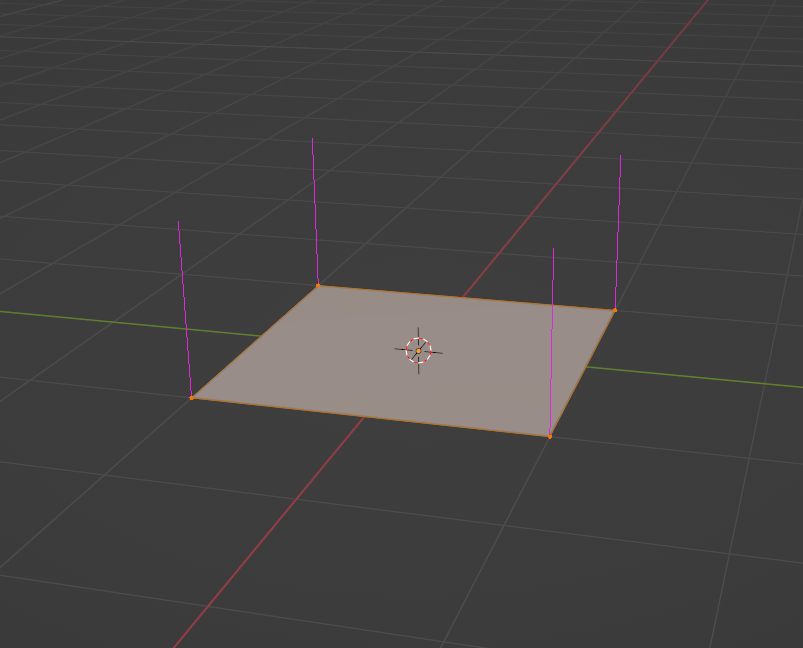
\includegraphics[scale=0.40]{images/ChBlinnPhong/QuadVertexNormals.png}
    \caption{Quad vertex normals visualization}
    \label{fig::QuadVertexNormals}
\end{figure}

\begin{figure}[ht]
    \centering
    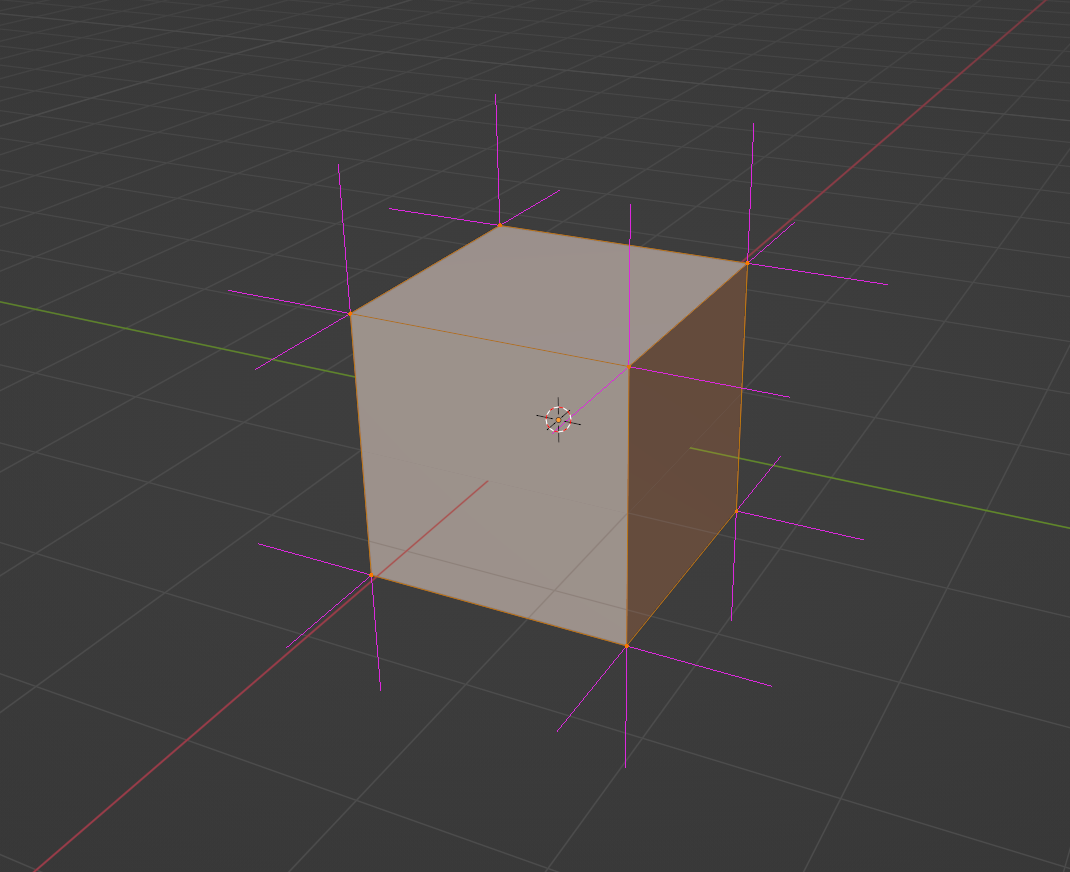
\includegraphics[scale=0.30]{images/ChBlinnPhong/CubeVertexNormals.png}
    \caption{Cube vertex normals visualization}
    \label{fig::CubeVertexNormals}
\end{figure}

\section{Blinn-Phong Lighting Model}

In computer graphics, lighting is approximated using simplified models.
The lighting model we use is called Blinn-Phong.
This model divides light into three components: ambient light, diffuse light and
specular light.

\section{Ambient Lighting}

Even when there is no apparent light source, objects aren't completely dark.
This is because some light can come from distant light sources.
To simulate this we use a constant that always gives the object some color.

In the real world, light comes from different sources around us, even if they
are not directly visible.
This is due to the fact that light scatters and bounces in different directions.
Hence, some light sources can have an indirect impact on the lighting of an object.

To simulate this light property, we use a small constant light value that we
add to our objects' lighting.
To add ambient lighting to a scene, we take the light's color, multiply it with
an ambient factor and multiply the result with the object's color.
This is our object's fragments color.

\begin{minipage}{\linewidth}{\noindent}
    \lstinputlisting[
        language=C++,
        caption={Computing ambient component},
        label={lst::ShadeAmbient}
        ]{src/ChBlinnPhong/ShadeAmbient.frag}
\end{minipage}

\begin{figure}[ht]
    \centering
    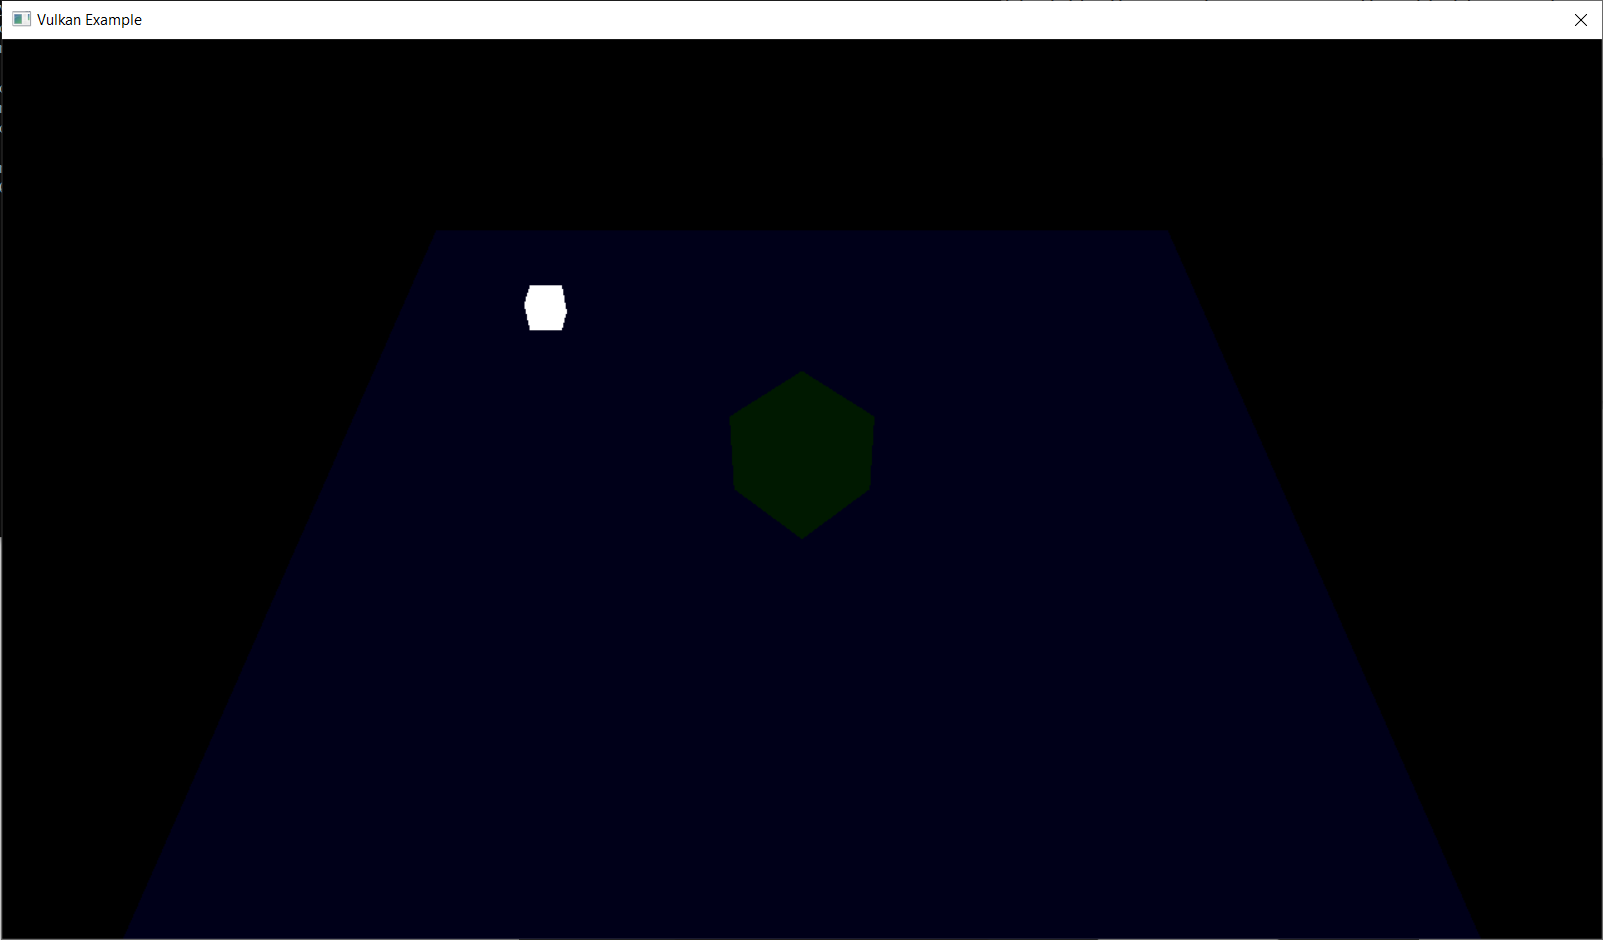
\includegraphics[scale=0.25]{images/ChBlinnPhong/SceneAmbient.png}
    \caption{Scene with ambient lighting}
    \label{fig::SceneAmbient}
\end{figure}

\section{Diffuse Lighting}

Diffuse lighting simulates the impact a light has on an object.
In simple terms, the more a part of the object faces the light, the brighter
it becomes.

Diffuse lighting gives the object more brightness the closer its fragments
are aligned to the light rays.

To compute the diffuse impact of the light on the fragment we take the dot
product between the surface's normal and the light direction.
The result is then multiplied with the light's color to get the diffuse component.
The greater the angle between the two vectors, the darker the diffuse component.

If the angle between the two vectors is greater than $90$ degrees, then the
diffuse impact will be negative.
We don't want this to happen.
Thus, all negative results will produce a zero diffuse impacts.

\begin{figure}[ht]
    \centering
    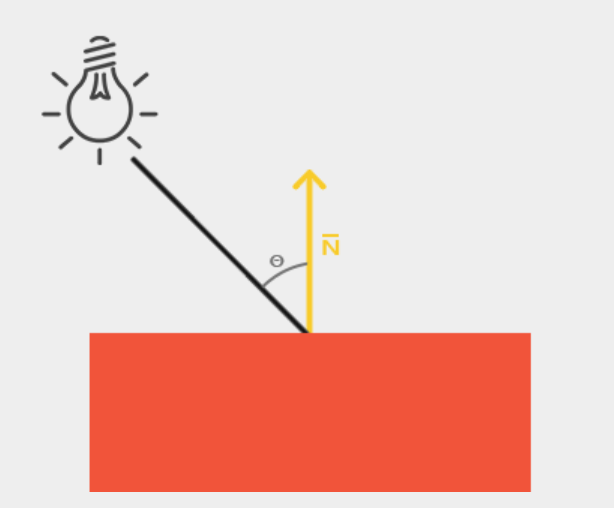
\includegraphics[scale=0.40]{images/ChBlinnPhong/DiffuseLighting.png}
    \caption{Computing diffuse lighting}
    \label{fig::ComputingDiffuseLighting}
\end{figure}

\begin{minipage}{\linewidth}{\noindent}
    \lstinputlisting[
        language=C++,
        caption={Computing diffuse component},
        label={lst::ShadeDiffuse}
        ]{src/ChBlinnPhong/ShadeDiffuse.frag}
\end{minipage}

\begin{figure}[ht]
    \centering
    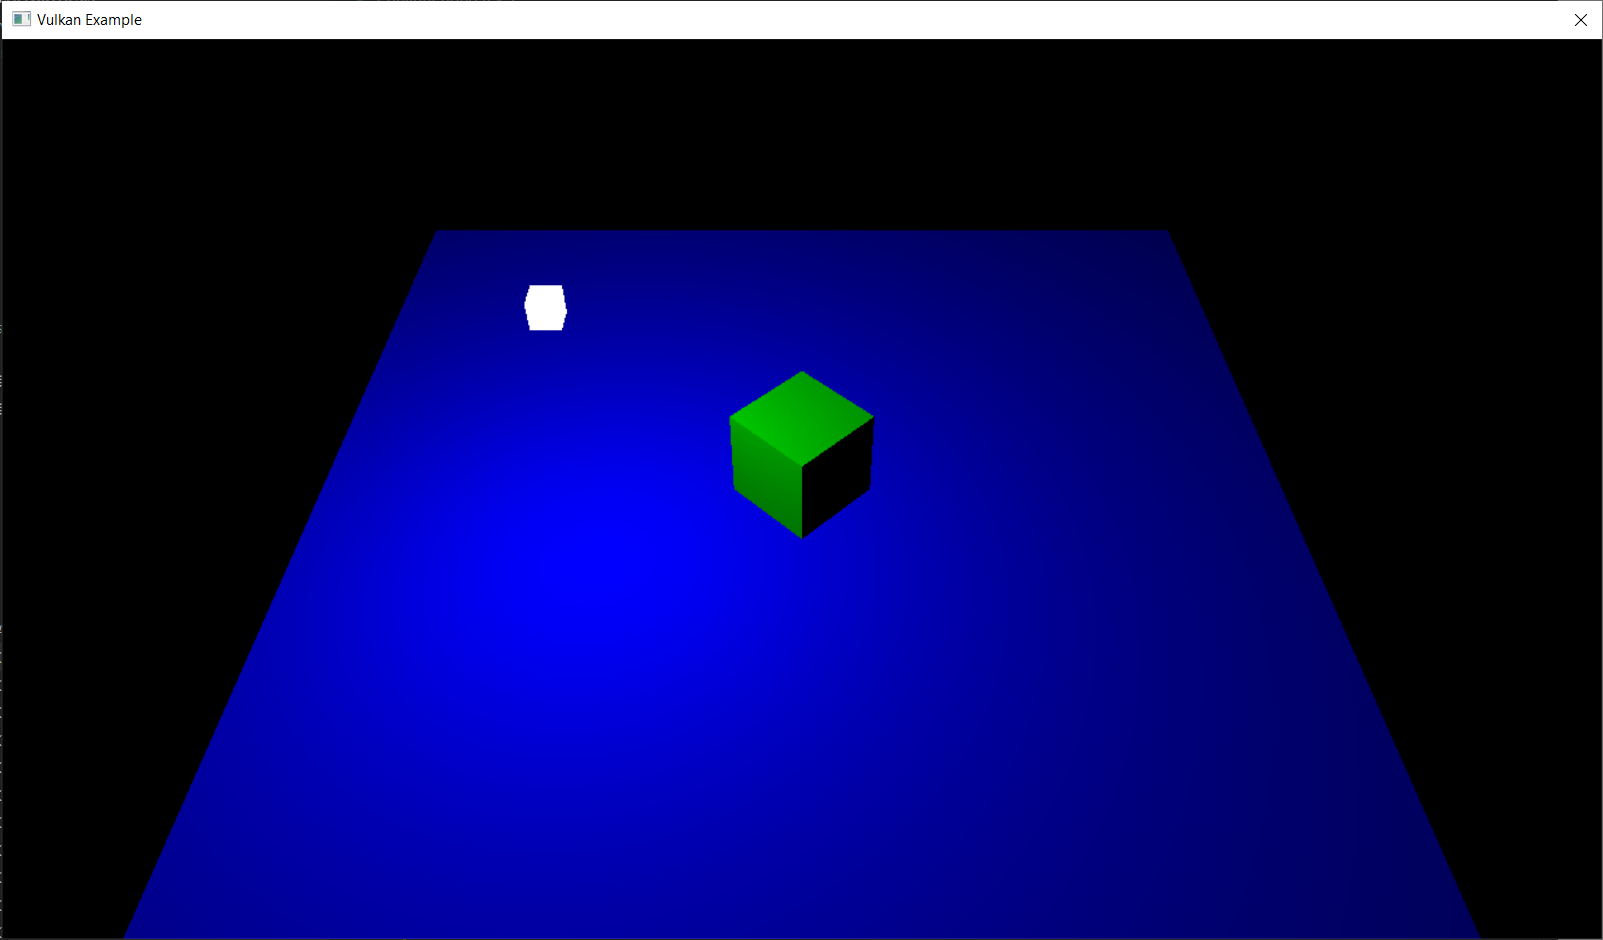
\includegraphics[scale=0.25]{images/ChBlinnPhong/SceneDiffuse.png}
    \caption{Scene with diffuse lighting}
    \label{fig::SceneDiffuse}
\end{figure}

\section{Specular Lighting}

Specular lighting simulates the bright spot that lights cause on bright objects.
This spot is called specular highlight.

Specular lighting is based on the reflective properties of surfaces.
Let's think of the object's surface as a mirror.
The specular impact is the strongest wherever we would see the light
reflected on the surface.

To compute the specular impact we first compute the halfway vector:
a unit vector exactly halfway between the view direction and the light direction.
The closer this halfway vector aligns with the surface's normal, the higher
the specular impact.

\begin{figure}[ht]
    \centering
    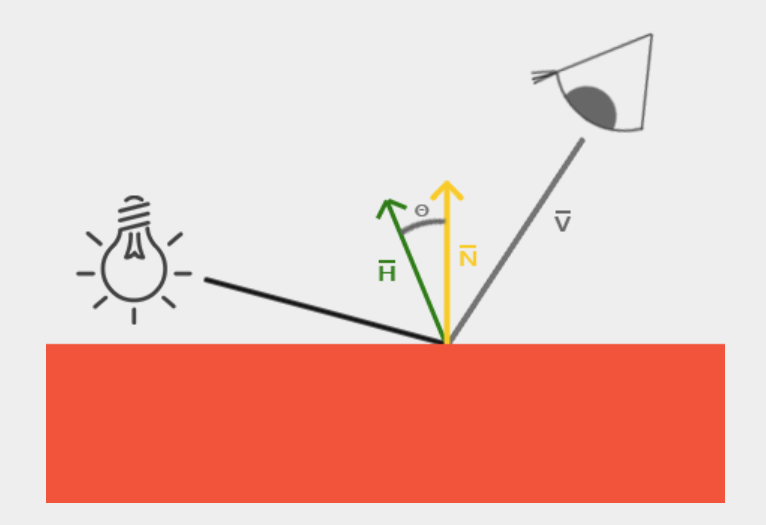
\includegraphics[scale=0.40]{images/ChBlinnPhong/SpecularLighting.png}
    \caption{Computing specular lighting}
    \label{fig::SpecularLighting}
\end{figure}

\begin{minipage}{\linewidth}{\noindent}
    \lstinputlisting[
        language=C++,
        caption={Computing specular component},
        label={lst::ShadeSpecular}
        ]{src/ChBlinnPhong/ShadeSpecular.frag}
\end{minipage}

\begin{figure}[ht]
    \centering
    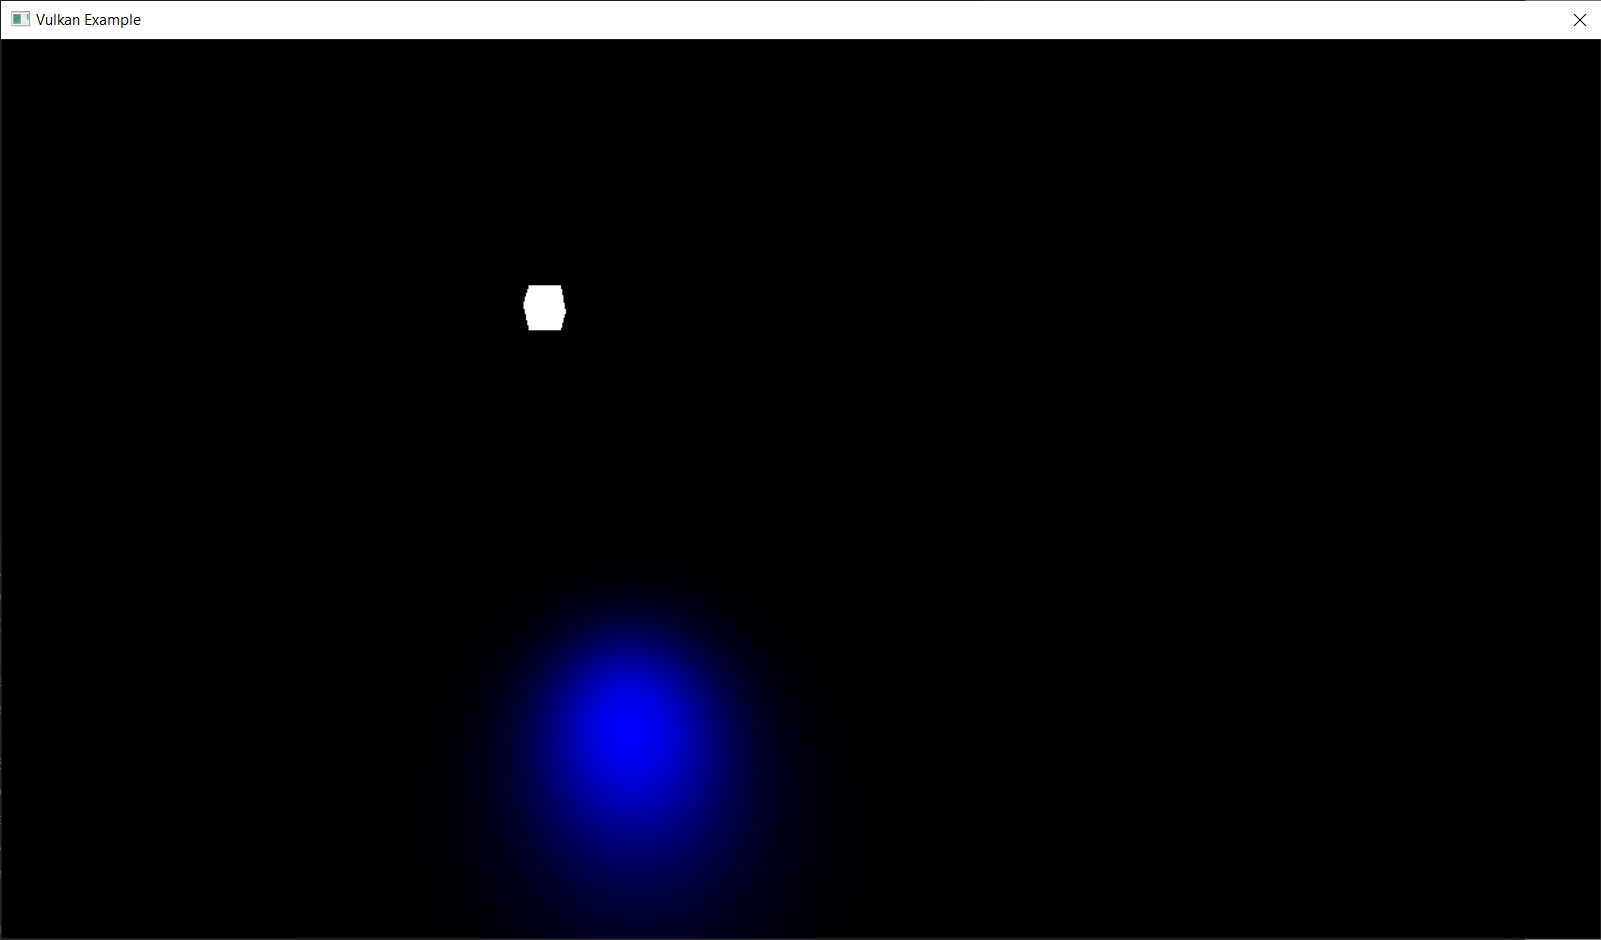
\includegraphics[scale=0.25]{images/ChBlinnPhong/SceneSpecular.png}
    \caption{Scene with specular lighting}
    \label{fig::SceneSpecular}
\end{figure}

\section{Putting It All Together}

\begin{figure}[ht]
    \centering
    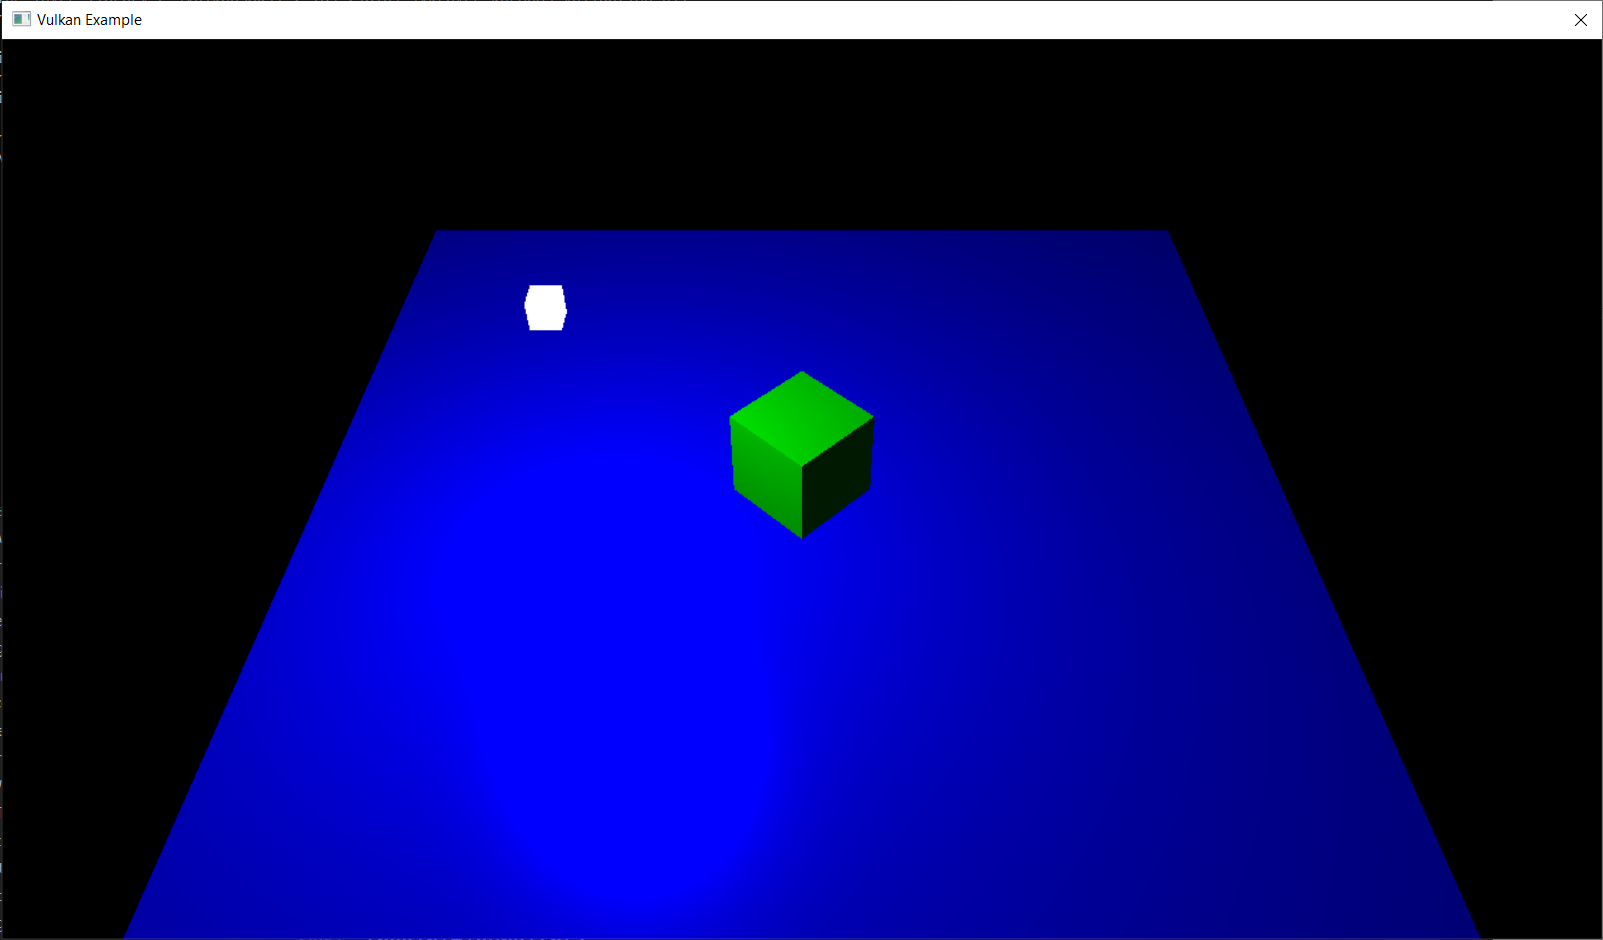
\includegraphics[scale=0.25]{images/ChBlinnPhong/SceneLit.png}
    \caption{Scene with ambient, diffuse and specular lighting}
    \label{fig::SceneLit}
\end{figure}

\section{Materials}

Real world objects have different reactions to light.
We simulate different types of objects using materials.
We can describe a material by specifying three different material colors,
one for each lighting component: ambient, diffuse and specular.
We also specify a material shininess property.
With these four components we can simulate a lot of real world materials.

The ambient material value defines what color the surface reflects under ambient
lighting.
This is usually the same as the surface's color.

The diffuse material value defines the color of the surface under diffuse lighting.

The specular material value defines the color of the specular highlight.

The shininess material value affects the specular highlight's radius.

Here we have given our floor a turquoise material.
Our cube uses a emerald material.

\begin{minipage}{\linewidth}{\noindent}
    \lstinputlisting[
        language=C++,
        caption={Materials used in our scene},
        label={lst::Materials}
        ]{src/ChBlinnPhong/Materials.cpp}
\end{minipage}

\begin{minipage}{\linewidth}{\noindent}
    \lstinputlisting[
        language=C++,
        caption={Blinn-Phong lighting using object materials},
        label={lst::ShadeMaterials}
        ]{src/ChBlinnPhong/ShadeMaterials.frag}
\end{minipage}

\begin{figure}[ht]
    \centering
    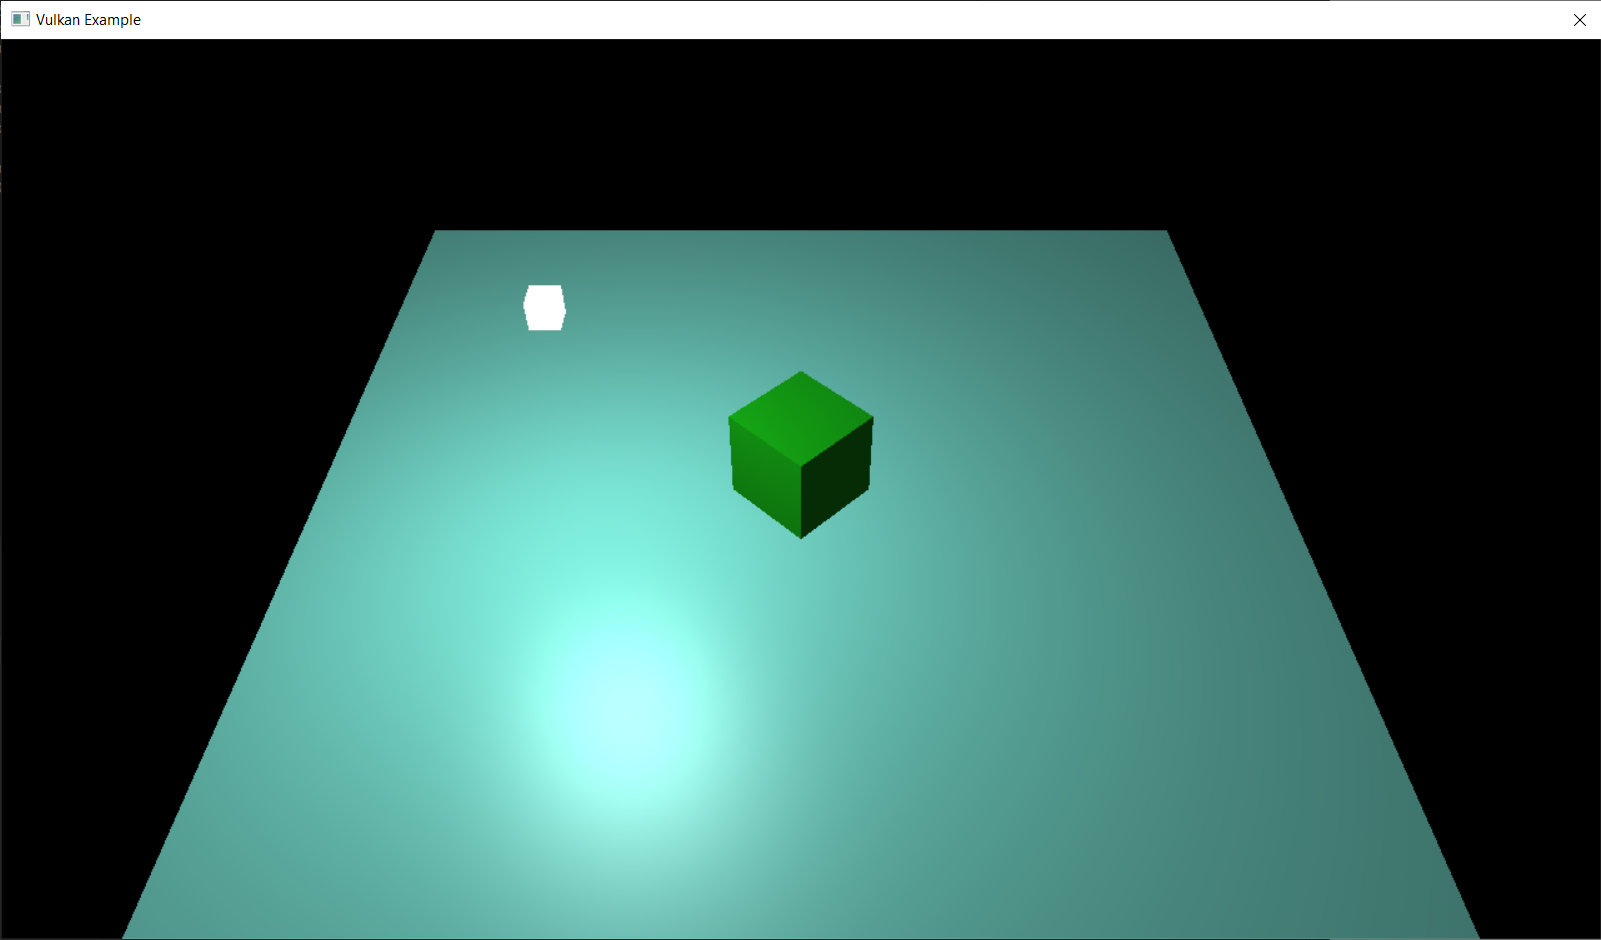
\includegraphics[scale=0.25]{images/ChBlinnPhong/SceneMaterials.png}
    \caption{Scene lighting using material properties}
    \label{fig::SceneMaterials}
\end{figure}

\section{Light Properties}

We can see that the objects are a little bit too bright.
This is due to the fact that the ambient, diffuse and specular colors are reflected
with full force from any light source.

Light sources also have different intensities for their ambient, diffuse and
specular components.

The ambient light is usually set to a low intensity because we don't want the
ambient color to be too dominant.

The diffuse component of a light source is usually set to the exact
color we'd like a light to have; often a bright white color.

The specular component is usually kept at vec3(1.0) shining at full intensity.

\begin{minipage}{\linewidth}{\noindent}
    \lstinputlisting[
        language=C++,
        caption={Our scene light's material},
        label={lst::LightMaterial}
        ]{src/ChBlinnPhong/LightMaterial.cpp}
\end{minipage}

\begin{minipage}{\linewidth}{\noindent}
    \lstinputlisting[
        language=C++,
        caption={Blinn-Phong lighting using object and light materials},
        label={lst::ShadeLightMaterial}
        ]{src/ChBlinnPhong/ShadeLightMaterial.frag}
\end{minipage}

\begin{figure}[ht]
    \centering
    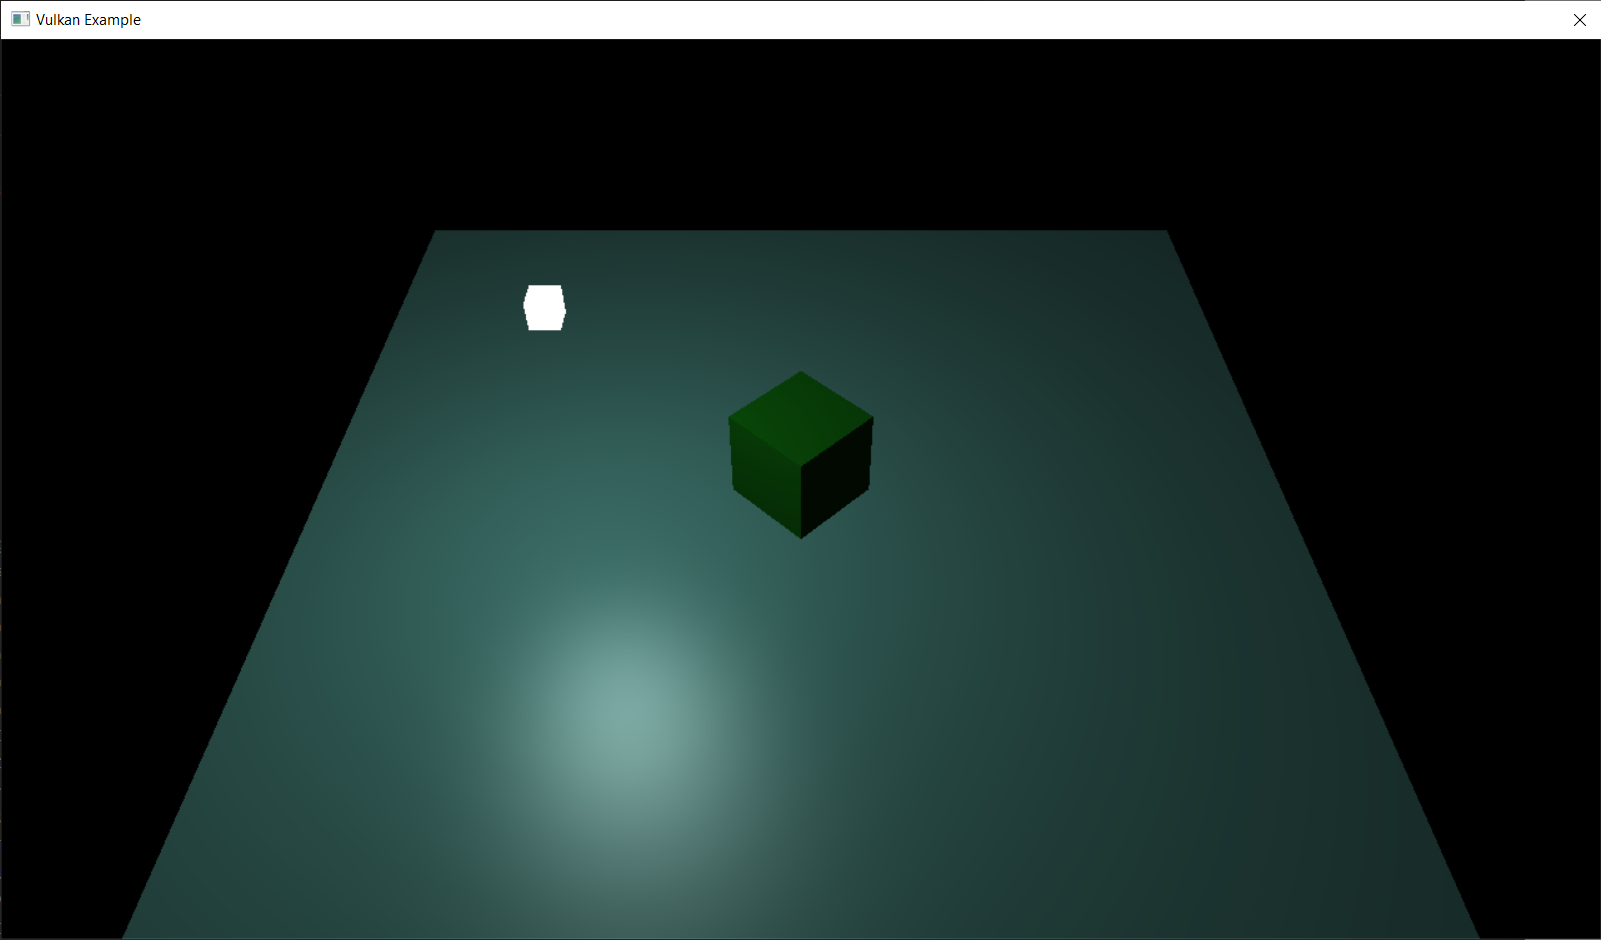
\includegraphics[scale=0.25]{images/ChBlinnPhong/SceneMaterialsLight.png}
    \caption{Scene lighting using object and light materials}
    \label{fig::SceneMaterialsLight}
\end{figure}
